\section{深入理解Ed25519}

\subsection{Ed25519概述}

Edwards-curve Digital Signature Algorithm (EdDSA)是定义在
(扭曲)爱德华曲线上Schnorr签名的变种签名机制.
Ed25519是Bernstein等人2011年在扭曲爱德华椭圆曲线Edwards25519 
(与蒙哥马利曲线Curve25519双向有理等价)上构建的签名机制\footnote{
Bernstein, Daniel J., Niels Duif, Tanja Lange, Peter Schwabe, and Bo-Yin Yang. 
"High-speed high-security signatures." 
In International Workshop on Cryptographic Hardware and Embedded Systems, 
pp. 124-142. Springer, Berlin, Heidelberg, 2011.
\url{https://link.springer.com/content/pdf/10.1007/978-3-642-23951-9_9.pdf}},
显著特点是高效安全,在保证128比特的安全强度的前提下
在2.4GHz的Intel Westmere (Xeon E5620) CPU上可以达到10万/秒的签名速度和7万/秒的验签速度.
RFC 8032\footnote{
RFC 8032. Edwards-Curve Digital Signature Algorithm (EdDSA).
\url{https://tools.ietf.org/html/rfc8032}}
中给出了EdDSA签名的具体规范,
并且给出了基于两条具体曲线Edwards25519和Edwards448的签名机制Ed25519和Ed448测试向量.
其中Edwards448是Mike Humberg构建的椭圆曲线,旨在提供224比特的安全强度.
值得注意的是, 2015年Bernstein对EdDSA签名机制进行了推广\footnote{
Bernstein, Daniel J., Simon Josefsson, Tanja Lange, Peter Schwabe, and Bo-Yin Yang. 
"EdDSA for more curves." Cryptology ePrint Archive 2015 (2015).
\url{https://eprint.iacr.org/2015/677.pdf}}
以使EdDSA签名机制可以适用于更多的椭圆曲线.
本文中,我们重点关注基于Edwards25519曲线的EdDSA的变种形式
\textsf{PureEdDSA}和\textsf{HashEdDSA}的签名机制:\textsf{Ed25519}和\textsf{Ed25519ph}.
RFC 8032中为了统一两个变种的定义,引入了预哈希函数(Prehash) \textsf{PH}的参数.
HashEdDSA是经典的先计算哈希值然后对哈希值计算签名的模式,也即对于任意长度的消息$m$,
\textsf{PH}都会输出固定长度的哈希值,例如\textsf{PH}可以定义为\textsf{SHA-512}: 
$\textsf{PH}(m) = \textsf{SHA-512}(m)$. PureEdDSA则直接对消息本身进行签名,
此时\textsf{PH}为恒等函数(Identity Function), 也即$\textsf{PH}(m) = m$.

EdDSA签名机制具有诸多良好的特性: 
1) 在各种平台上都可以高速实现; 2) 签名过程不需要外部随机数; 3) 能够有效抵抗侧信道攻击;
4) 公钥和签名值都较小,对于Ed25519而言公钥为32个字节签名值为64个字节;
5) 曲线上的点群运算是完备(Complete)的, 也即对于所有的点群中元素都成立, 计算时无需做额外的判断, 
意味着运算时不需要对不受信的外部值做昂贵的点的验证; 
6) EdDSA签名机制本身安全性不受哈希碰撞的影响,而ECDSA在出现哈希碰撞时会出现安全问题.

\subsection{EdDSA签名机制}

根据Bernstein等人在2015年对EdDSA签名机制的推广和RFC 8032中的规范, EdDSA签名机制有11个参数:
\begin{enumerate}
\item 
奇素数$p$: EdDSA所依赖的椭圆曲线构建在有限域$\F_p$上.
\item 
整数$b$满足$2^{b-1} > p$: EdDSA公钥为$b$比特,签名值为$2b$比特, $b$应为8的整数倍.
\item
有限域$\F_p$中元素的$b-1$比特的编码.
\item
可以产生$2b$比特输出的具有密码学安全强度的哈希函数\textsf{H}.
\item
$\F_p$中的二次非剩余$d$, $d$是椭圆曲线方程的参数,推荐选择尽可能接近零的值.
\item
$\F_p$中非零元素$a$, $a$是曲线方程参数, 推荐$p \mod 4=1$取$a=-1$, 否则取$a=1$.
\item 
基点$B \neq (0, 1)$并且$B \in E = \{(x,y) \in \F_p \times \F_p\ s.t.\ ax^2 + y^2 = 1 + dx^2y^2\}$.
\item
整数$c = 2$或$c = 3$, $2^c$是椭圆曲线的余因子(cofactor), EdDSA私钥为$2^c$的倍数.
\item
整数$n$满足$c \leq n < b$, 私钥为$n+1$比特,最高位为1 ($2^n$位),最低$c$位置零.
\item
奇素数$\ell$满足$\ell B = (0,1)$并且$2^c \times \ell = \# E$, 即$\ell$为椭圆曲线点群的阶(Order).
\item
预哈希函数\textsf{PH}, \textsf{PureEdDSA}和\textsf{HashEdDSA}对\textsf{PH}的定义不同.
\end{enumerate}
点群中的单位元为$(0,1)$,并且点群上的加法运算是完备的(Complete), 
也即对于任意的点$(x_1,y_1), (x_2, y_2)$都有
$$(x_1, y_1) + (x_2, y_2) = \left( \frac{x_1y_2 + x_2y_1}{1 + dx_1x_2y_1y_2}, 
\frac{y_1y_2 - ax_1x_2}{1-dx_1x_2y_1y_2}\right)$$

整数$s: 0 < s < \ell - 1$用小端法编码为$b$比特的字符串的过程记为$\textsf{Encode}(s)$.
而$(x,y)\in E$被编码为$b$比特的字符串,记为$\textsf{Encode}(x,y)$, $b$比特的编码
包含$y$的$(b-1)$比特的编码和1比特的符号位:如果$x$是负数, 则符号位为1, 否则为0.
根据这种编码方式可以立即确定$y$的值, $x$的值则需要通过方程
$x = \pm\sqrt{(y^2-1)/(dy^2-a)}$和符号位进行确定
(由于$d$是$\F_p$中的二次非剩余,所以分母$dy^2-a$不为零).
$x, y \in \F_p$, EdDSA签名体制中对有限域$\F_p$中的负数的定义为:
如果$x$的$(b-1)$比特的编码字符串比$-x$的$(b-1)$比特的编码字符串字典序更大
(Lexicographically Larger),则$x\in\F_p$是负数.
对于$p$是大的奇素数并且采用小端法编码的情形, $\F_p$中负数是所有的奇数$\{1, 3, 5, \ldots, q-2\}$.

EdDSA签名机制的私钥是$b$比特的值$k$, 记$\textsf{H}(k) = (h_0, h_1, \ldots, h_{2b-1})$.
$h_0, h_1, \ldots, h_{b-1}$确定了一个整数值$s$:
$$s =  2^n + \sum_{c \leq i < n}2^i h_i$$
整数值$s$决定公钥$\textsf{Encode}(A)$, 其中$A = sB$.
$h_b, h_{b+1}, \ldots, h_{2b-1}$用在签名值的计算过程中.
前面有提到, RFC 8032中根据预哈希函数\textsf{PH}的定义了给出了EdDSA的两个变种:
\textsf{PureEdDSA}和\textsf{HashEdDSA}, 由于两者的差异仅在于用\textsf{PH}处理
待签名消息$m$的结果不同,因此EdDSA可描述为:用\textsf{PureEdDSA}对$\textsf{PH}(m)$进行签名.

\textsf{PureEdDSA}对消息$m$计算签名值的结果$2b$比特的值
$\textsf{Encode}(R) || \textsf{Encode}(S)$: 
$$R = rB, S = \left(r + \textsf{H}\left(\textsf{Encode}(R) || 
\textsf{Encode}(A) || \textsf{PH}(m)\right)\cdot s \right) \mod \ell$$
其中$r = \textsf{H}(h_b || \ldots || h_{2b-1} || m)$并且被解释为小端法表示的$2b$比特的整数值.
用公钥值$\textsf{Encode}(A)$验证关于消息$m$的签名值$\textsf{Encode}(R) || \textsf{Encode}(S)$时,
首先需要从中解析出$A, R, S$的值,
并判定$A$和$R$是$E$中的元素并且$S$是集合$\{0, 1, \ldots, \ell-1\}$中的值,
然后判断如下等式是否成立
$$
(2^c \cdot S) B = 2^c  R + (2^c \cdot h) A,
\ \text{其中}\ h = \textsf{H}(\textsf{Encode}(R) || \textsf{Encode}(A) || \textsf{PH}(m))
$$
如果解析失败或者上述等式不成立,则判定为非法的签名值,否则判定为合法的签名值.
对消息$m$的EdDSA签名值的验证过程也即用\textsf{PureEdDSA}对$\textsf{PH}(m)$的签名值的验证过程.

\textsf{Ed25519}/\textsf{Ed25519ph}是基于扭曲爱德华曲线Edwards25519实例化的EdDSA签名机制, 
对应前述的EdDSA签名机制的11个参数分别为: 
\begin{enumerate}
\item 有限域$\F_p$的奇素数$p = 2^{255} - 19$.
\item 整数$b  = 256$, 也即\textsf{Ed25519}的公钥为256比特,签名值为512比特,注意到$2^{255} > p$.
\item $\F_p$中元素$\{0, 1, \ldots, p-1\}$的255比特编码是用小端法表示的整数值,最高位为零.
\item 
基于\textsf{SHA-512}\footnote{
RFC 6234: US Secure Hash Algorithms (SHA and SHA-based HMAC and HKDF).
\url{https://tools.ietf.org/pdf/rfc6234.pdf}}
的生成512比特输出的哈希函数$\textsf{SHA-512}(\textsf{dom2}(f, c) || x)$.
$f$是$flag$缩写,而$c$是$context$的缩写.
对于\textsf{Ed25519}, $\textsf{dom2}(f, c)$是空字符串, 也因此$f$和$c$的值无关紧要,
这样可以保证RFC 8032中定义的$\textsf{Ed25519}$与已有的$\textsf{Ed25519}$实现之间保持兼容. 
\textsf{Ed25519ctx}和\textsf{Ed25519ph}都可以带有额外的上下文参数$c$,至多为255个字节,
对于\textsf{Ed25519ctx}而言, $f = 0$, 对\textsf{Ed25519ph}而言, 则有$f = 1$. 
\item $\F_p$中的二次非剩余$d = -121665/121666$.
\item 由于$2^{255}-19 \mod 4 = 1$, 因此选取$\F_p$中的非零元素$a = -1$.
\item 基点$B$的横坐标\small{\textsf{0x216936d3cd6e53fec0a4e231fdd6dc5c692cc7609525a7b2c9562d608f25d51a}},
\normalsize
纵坐标为\small{\textsf{0x6666666666666666666666666666666666666666666666666666666666666658}}.
\normalsize
\item Edwards25519的余因子为8, 也因此整数参数$c = 3$.
\item $n = 254$.
\item Edwards25519的阶$\ell = 2^{252}+27742317777372353535851937790883648493$.
\item \textsf{Ed25519}的预哈希函数定义为\textsf{PH}为恒等函数, \textsf{Ed25519ph}的\textsf{PH}定义为\textsf{SHA-512}.
\end{enumerate}

由于Edwards25519的点坐标的值位于$\F_p$中, 根据$\F_p$中元素的255比特,可以用32字节的值
编码点$(x,y)$: 用255比特的值编码$y$的值,由于采用小端法编码,则32字节中的最后一个字节的最高位为零)
然后将$x$的最低比特赋值给最后一个字节的最高位即可. 这是因为最后一个字节的最高比特位是符号位,
符号位为1表示$x$为负值, 根据前述的关于$\F_p$中负数的定义可知, $\F_p$中的奇数均为负数, 
由于奇数的最低位为1, 所以将$x$的最低位赋值给符号位正好符合关于编码和负值的约定.

从32字节的编码中解码出点的值的步骤较编码复杂一些. 根据255比特的小端法编码可以直接得到$y$的值,
同时检查$y$的值在合理的范围之内并拒绝非法的值,而根据符号位可知$x$的最低位$x_0$.
根据$y$和曲线方程得到的$x^2 = (y^2-1) / (dy^2 + 1) (\mod p)$可以恢复$x$的值, 计算中会涉及到
域上的求逆运算和域上的开平方运算.求逆可以利用费马小定理$x^{-1} = x^{p-2} \mod p$
或者扩展的欧几里得算法完成.

记$u = y^2-1, v = dy^2 + 1$, 考虑根据$x^2 = u/v \mod p$计算$x$的值.
根据欧拉准则(Euler's Criterion),
如果$u/v$是$\F_p$中的二次剩余,则有$(u/v)^{(p-1)/2} \equiv 1 \mod p$;
如果$(u/v)^{(p-1)/2} \equiv -1 \mod p$, 则$x^2 = u/v \mod p$无解.
考虑$u/v$是$\F_p$中二次剩余的情况, 
注意到$2^{255}-19 \equiv 5 \mod 8$, 也即存在整数$k$使得$p = 8k + 5$.
由于$(u/v)^{(p-1)/2} \equiv 1 \mod p$, 则有$(u/v)^{(p-1)/4} \equiv \pm 1 \mod p$.
如果$(u/v)^{(p-1)/4} \equiv 1 \mod p$, 则$x = (u/v)^{k+1}\mod p$是一个解:
$$
x^2 \equiv (u/v)^{2(k+1)} \equiv (u/v)^{(p+3)/4} \equiv (u/v)^{(p-1)/4}\cdot (u/v) \equiv (u/v) \mod p 
$$
如果$(u/v)^{(p-1)/4} \equiv -1 \mod p$, 则$x = 2^{2k+1}(u/v)^{k+1}\mod p$是一个解:
$$
x^2 \equiv 2^{4k+2}(u/v)^{2k+2} \equiv 2^{\frac{p-1}{2}}(u/v)^{\frac{p+3}{4}} \equiv
 2^{\frac{p-1}{2}} (u/v)^{\frac{p-1}{4}}\cdot (u/v) \equiv -1 \cdot -1 \cdot (u/v) \mod p
$$
上式成立的原因在于2是$\F_p$中的二次非剩余以及欧拉准则$2^{(p-1)/2}\equiv -1 \mod p$.

根据上述过程,继续描述从32字节的编码中解码出点坐标值的过程,从$y$的值可以计算出$u, v$的值.
当$u/v$是$\F_p$中的二次剩余时,计算$x \equiv (u/v)^{(p+3)/8}\mod p$,
如果$x^2 \equiv (u/v) \mod p$, 则$x$是平方根,
如果$x^2 \equiv -(u/v)\mod p$, 则$2^{(p-1)/4} \cdot x$ (也即$\sqrt{-1}\cdot (u/v)^{(p+3)/8}$)是平方根,
否则$u/v$不是$\F_p$中的二次剩余,意味着解码失败.
下一步则根据$x_0$的值选取正确的平方根,如果$x = 0$而$x_0 = 1$, 则解码失败.
如果$x_0 \neq x \mod 2$, 则$x = p-x$, 解码得到的点即为$(x,y)$.
注意在具体实现解码操作时,可以将求逆和求平方根的操作进行融合以简化运算,
$(u/v)^{(p+3)/8}\mod p$可以等价变换为:
$$
(u/v)^{(p+3)/8} = u^{\frac{p+3}{8}} v^{-\frac{p+3}{8}}
= u^{\frac{p+3}{8}} v^{(p-1)-\frac{p+3}{8}}
= u^{\frac{p+3}{8}} v^{\frac{7p-11}{8}}
= uv^3(uv^7)^{(p-5)/8} 
$$
而判断$x^2\equiv (u/v) \mod p$和$x^2 \equiv -(u/v) \mod p$可以等价变换为
$v \cdot x^2 \equiv u \mod p$和$v \cdot x^2 \equiv -u \mod p$.

与secp256k1或者secp256r1等曲线的实现时常采用的Jacobi坐标系$(X, Y, Z), x = X/Z, y = Y/Z$等不同, 
Hisil等人指出\footnote{
Hisil, Huseyin, Kenneth Koon-Ho Wong, Gary Carter, and Ed Dawson. 
"Twisted Edwards curves revisited." 
In International Conference on the Theory and Application of Cryptology and Information Security, 
pp. 326-343. Springer, Berlin, Heidelberg, 2008.
\url{https://eprint.iacr.org/2008/522.pdf}}对于扭曲爱德华曲线Edwards25519,
采用扩展的扭曲爱德华坐标系(Extended Twisted Edwards Coordinates)表示
$(x,y) \rightarrow (X : Y : Z : T), x = X/Z, y = Y/Z, T = XY/Z, Z \neq 0$更有利于点运算的高效实现.
在扩展的扭曲爱德华坐标系下, 单位元为$(0 : 1 : 1 : 0)$, $(X : Y : Z : T)$的逆元为$(-X : Y : Z : -T)$.
判断两个点$(X_1, Y_1, Z_1, T_1), (X_2, Y_2, Z_2, T_2)$相等等价于判断
$X_1/Z_1 = X_2/Z_2\ \&\ Y_1/Z_1 = Y_2/Z_2$, 由于素数域上的求逆运算需要较多的计算量,
为了避免求逆运算并且注意到$Z_1 \neq 0, Z_2 \neq 0$, 前述判断可以等价变换为
$X_1 \cdot Z_2 = X_2 \cdot Z_1\ \& \ Y_1 \cdot Z_2 = Y_2 \cdot Z_1$.
而两个点的加法运算$(X_1, Y_1, Z_1, T_1) +  (X_2, Y_2, Z_2, T_2) = (X_3, Y_3, Z_3, T_3)$,
可以按照如下步骤进行, 值得注意的是如下计算步骤对于两个点相同的情况同样适用.
\begin{equation*}
\begin{array}{c}
A \leftarrow (Y_1 - X_1) \cdot (Y_2 - X_2), B \leftarrow (Y_1 + X_1) \cdot (Y_2 + X_2) \\
C \leftarrow 2\cdot T_1 \cdot T_2, D \leftarrow 2 \cdot Z_1 \cdot Z_2 \\
E \leftarrow B - A, F \leftarrow D - C, G \leftarrow D + C, H \leftarrow B + A \\
X_3 \leftarrow E \cdot F, Y_3 \leftarrow G\cdot H, T_3 \leftarrow E \cdot H, Z_3 \leftarrow F \cdot G
\end{array}
\end{equation*}

Listing~\ref{lst-ed25519point}~中展示了基于扩展的扭曲爱德华坐标系实现的点的加法, 加倍以及倍乘运算
,参见函数~\code{point_add}, \code{point_double}~以及~\code{point_mul}.
同时展示了前述的点的编解码过程(参见函数~\code{point_compress}~和~\code{point_decompress})
以及判断两个点是否相同的函数~\code{point_equal}.
\code{point_decompress}~过程中所需的恢复横坐标的运算,在函数~\code{recover_x}~中实现.
函数~\code{point_mul}~内部实现点的倍乘运算时,采用了经典的double-and-add方法.

\lstinputlisting[firstline=1, lastline=95, language=python, 
caption=\texttt{Edwards25519点运算与编解码}, label=lst-ed25519point]{ed25519.py}

与ECDSA签名机制中直接用私钥和基点进行点倍乘运算得到公钥值不同,
EdDSA签名机制中私钥和公钥之间的关系更为复杂,按照以下步骤进行(参见Figure~\ref{fig-ed25519}):
1) 用\textsf{SHA-512}计算32字节的私钥的512比特(64个字节)的哈希值,低32字节用于生成公钥;
2) 将32字节中第一个字节的最低3比特清零,最后一个字节的最高位清零,将最后一个字节的第二最高位置1;
3) 将设置之后的32字节的看做是小端法表示的整数,记为$s$, 计算$A = sB$;
4) $A$的编码$\textsf{Encode}(A)$是最终的公钥.

\begin{figure}[h]
\centering
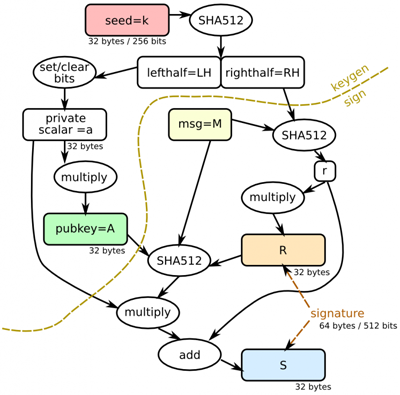
\includegraphics[width=.7\textwidth]{ed25519.png}
\caption{Ed25519签名过程}\label{fig-ed25519}
\end{figure}

签名过程先利用\textsf{SHA-512}对私钥进行哈希运算,得到64字节的输出,
记为$h = (h[0], h[1], \ldots, h[63])$, 其中$h[i], i \in \{0, 1, \ldots, 63\}$表示第$i$个字节.
如前所述$(h[0], \ldots, h[31])$用于生成公钥值, 记$prefix = h[32] || h[33] || \ldots || h[63]$, 
$prefix$在后续的EdDSA签名过程中扮演了随机数的角色.
计算
$$\textsf{SHA-512}(\textsf{dom2}(F, C) || prefix || \textsf{PH}(m)),$$
其中根据\textsf{Ed25519}, \textsf{Ed25519ctx}, \textsf{Ed25519ph}的不同,
$\textsf{dom2}(F,C)$和$\textsf{PH}(m)$的定义有所不同,
得到的64字节的哈希值解释为小端法表示的整数$r$并计算
$$R = rB.$$
计算
$$\textsf{SHA-512}\left(\textsf{dom2}(F,C) || \textsf{Encode}(R) || \textsf{Encode}(A) || \textsf{PH}(m)\right).$$
将得到的64字节的哈希值解释为小端法表示的整数$k$并计算
$$ S = (r + k * s) \mod \ell.$$
最终的签名值为32字节的$\textsf{Encode}(R)$以及32字节的$\textsf{Encode}(S)$,总计为64字节.

签名验证时从签名值$\textsf{Encode}(R)||\textsf{Encode}(S)$解码得到点$R$和整数$S$,
解码$\textsf{Encode}(A)$得到公钥点$A$.
如果签名值或者公钥值解码失败或者$S$的值不在合理的范围内,则判定为非法的签名值.
计算
$$\textsf{SHA-512}\left(\textsf{dom2}(F,C) || \textsf{Encode}(R) || \textsf{Encode}(A) || \textsf{PH}(m)\right).$$
将得到的64字节的哈希值解释为小端法表示的整数$k$并检查下面的等式是否成立:
$$(8S)B = 8R + (8k)A.$$
若等式成立,则判定为合法的签名值; 否则判定为非法的签名值.
\textsf{Ed25519}签名验签的Python示例代码参见Listing~\ref{lst-ed25519},
其中函数~\code{secret_to_pubkey}~实现从私钥生成公钥的过程,
函数~\code{ed25519_sign}~和~\code{ed25519_verify}~则分别实现了Ed25519的签名和验签.

\lstinputlisting[firstline=97, lastline=142, language=python, 
caption=\texttt{Ed25519签名机制}, label=lst-ed25519]{ed25519.py}

根据Listing~\ref{lst-ed25519point}~和Listing~\ref{lst-ed25519}~中的Python示例代码,
配合RFC 8032中给出的测试向量,可以验证PoC代码的正确性,参见Listing~\ref{lst-ed25519check}.

\begin{lstlisting}[language=python, caption=验证Ed25519实现正确性, label=lst-ed25519check]
>>> import ed25519
>>> import base64
>>>
>>> secret_str = (
... '9d61b19deffd5a60ba844af492ec2cc4'
... '4449c5697b326919703bac031cae7f60')
>>> pubkey_str = (
... 'd75a980182b10ab7d54bfed3c964073a'
... '0ee172f3daa62325af021a68f707511a')
>>> msg_str = ""
>>> sig_str = (
... 'e5564300c360ac729086e2cc806e828a'
... '84877f1eb8e5d974d873e06522490155'
... '5fb8821590a33bacc61e39701cf9b46b'
... 'd25bf5f0595bbe24655141438e7a100b')
>>>
>>> secret = base64.b16decode(secret_str, True)
>>> pubkey = base64.b16decode(pubkey_str, True)
>>>
>>> msg    = base64.b16decode(msg_str, True)
>>> sig    = base64.b16decode(sig_str, True)
>>> 
>>> pubkey == ed25519.secret_to_pubkey(secret)
True
>>> base64.b16encode(ed25519.ed25519_sign(secret, msg)).lower()
b'e5564300c360ac729086e2cc806e828a84877f1eb8e5d974d873e0652249015
58d87fc207b0549fb6bc61bf6b550c7875e5f2a43320abd01ee6f2ef6965e5829'
>>>
>>> ed25519.ed25519_verify(pubkey, msg, sig)
True
\end{lstlisting}

\subsection{几种签名机制的关系}

EdDSA签名机制中的验签中判断的核心等式是$(2^c\cdot S)B = 2^c R + (2^c\cdot h)A$,
其中每个点倍乘的标量都乘以$2^c$的原因是为了应对余因子不为1可能带来的安全隐患.
如果不考虑标量中的$2^c$, 则这个等式与Schnorr签名机制中验签判定的核心等式基本一致.
关于这点Bernstein等人在提出EdDSA签名机制的论文中就ElGamal,  (EC-)Schnorr, 
(EC-)DSA以及EdDSA签名机制之间的联系有着精彩的论述.

ElGamal签名机制是在椭圆曲线密码学诞生之前提出的,工作在大素数乘法群$\Z^*_p$上,
阶为$\ell = p-1$, 本原元记为$B$, 私钥记为$a$, 公钥记为$A \equiv B^a \mod p$, 
则对消息$m$的在随机数$k \in\Z^*_{\ell}$下的签名值为$(R, S)$, 其中
$$R \equiv B^k \mod p, \ S \equiv k^{-1} \cdot (\textsf{H}(m) - Ra) \mod \ell.$$
签名验证涉及到的核心的判断是
$$B^{\textsf{H}(m)} \equiv A^R \cdot R^S \mod p.$$
对于正确的签名值有$A^R \cdot R^S \equiv B^{aR} B^{kS} \equiv B^{aR + kS} \mod p$,
又由于
$$S \equiv k^{-1} \cdot (\textsf{H}(m) - Ra) \mod \ell \implies aR + kS \equiv \textsf{H}(m) \mod \ell,$$
因此对于正确的签名值有$B^{\textsf{H}(m)} \equiv A^R \cdot R^S \mod p$成立.

为了满足安全性,现在通常推荐素数$p$需要为2048比特,则对应的ElGamal签名值为4096比特,
签名值较大. 1989年Schnorr提出了可以看做是ElGamal签名机制变种的Schonrr签名机制,
能够大大缩短签名值的长度. 而数字签名算法DSA是吸收了Schnorr签名设计思想的另一种ElGamal
签名机制的变种签名机制. DSA在1994年被采纳为FIPS标准: FIPS-186.
基于椭圆曲线的DSA方案即为熟知的ECDSA.

根据拉格朗日定理可知,大素数乘法群$\Z^*_p$存在阶为$q,\ q | (p-1)$的乘法子群.
对于$p\approx2^{1024}$的情况,一般取$q \approx2^{160}$.
Schnorr签名机制对ElGamal签名机制进行了改动,使得最终的签名值只有$2\log_2(q)$比特
而非$2\log_2(p)$. Schnorr签名工作在$\Z^*_p$中的$q$阶子群,
方案的安全性基于这样的事实: 在特定的$\Z^*_p$子群上求解离散对数问题是困难的.

ElGamal的签名验证过程中$R$扮演了两种角色: $\Z^*_p$中的元素以及$A$的指数.
由于群的元素不一定可以直接作为指数(标量),因此更广义的群结构通常需要一个将群中元素
映射成为标量的映射$\mathbf{x}$.例如ECDSA签名机制依赖的群结构是大素数域$\F_p$上的
椭圆曲线加法点群中阶为$\ell$的子群, 而映射$\mathbf{x}(R)$定义为点$R$的$x$坐标.
对比ElGamal签名机制, ECDSA签名机制中还用$-A$替换了$A$,则签名过程中的减法相应
变换为加法, 对于基点$B$, 私钥$a$, 公钥$A = aB$, 
消息$m$在随机数$k$下的签名值为$(\mathbf{x}(R),S)$, 其中:
$$R = kB, \ S = k^{-1}(\textsf{H}(m) + \mathbf{x}(R)a) \mod \ell.$$
并且签名验证中判断的主要方程变为: 
$$\textsf{H}(m)B + \mathbf{x}(R)A = SR.$$
通过添加约束要求$S$模$\ell$可逆($\ell$为素数时,非零$S$模$\ell$都可逆),则前述方程变换为
$$S^{-1}\left(\textsf{H}(m)B + \mathbf{x}(R)A\right) = R,$$
对比之下,可以发现验证所需的计算从原先的3次点倍乘运算减少为2次点倍乘运算.

%为了便于对比,基于映射$\mathbf{x}$重新表示加法形式的ElGamal签名机制,
%例如基于椭圆曲线加法点群的阶为$\ell$的加法子群构建的EC-ElGamal签名机制.
%$B$表示基点,私钥为$a$, 公钥为$A=aB$,用随机数$k$
%对消息$m$签名使用的随机数为$k$, 则EC-ElGamal签名机制的签名值为$(R,S)$, 其中
%$$R = kB, \ S = k^{-1} (\textsf{H}(m) - aR)
%接下来展示如何通过逐步改进ElGamal签名机制得到Schnorr签名机制.
\textcolor{blue}{
对于映射$\mathbf{x}$, Schnorr签名则采用了密码学安全的哈希函数,
借助于哈希函数的高效率,用最少的计算代价消除了可能隐藏在简单$\mathbf{x}$映射中的数学结构.
与前述的ECDSA签名类似, Schnorr签名的签名值为$(\mathbf{x}(R), S)$而非$(R,S)$.
给定签名值$(\mathbf{x}(R), S)$, 验证者验证下面的等式是否成立:
$$\mathbf{x}(R') = \mathbf{x}(R),\ \text{其中}\ R' = S^{-1}(\textsf{H}(m)B + \mathbf{x}(R)A) .$$
Schnorr同时合并了对$R$和消息$m$的哈希计算$\textsf{H}(R||m)$, Bernstein等人指出
合并$R$和消息$m$的哈希计算可以理解成用$\mathbf{x}(R)S$替换$S$.
对于合法的Schnorr签名值,有等式$SR = \textsf{H}(m)B + \mathbf{x}(R)A$成立.
用$\mathbf{x}(R)S$替换$S$并假设$\mathbf{x}(R)\neq0$则有:
$$\mathbf{x}(R)SR = \textsf{H}(m)B + \mathbf{x}(R)A \implies 
SR = \mathbf{x}(R)^{-1}\textsf{H}(m)B + A.$$
注意到这里$\mathbf{x}(R)^{-1}\textsf{H}(m)$只是将两个哈希值做了乘法,
考虑$\textsf{H}(R||m)$时, $\mathbf{x}(R)^{-1}\textsf{H}(m)$是多余的,
则上式,也即签名验证的方程,可简化为$SR = \textsf{H}(R||m)B + A$.
签名过程中$S$的计算方式也调整成$S \equiv k^{-1}(\textsf{H}(R||m) + a) \mod \ell$,
仍然需要在签名时计算素数域上元素的逆.
Schnorr签名中真正利用的验证等式实际为$SB = R+ \textsf{H}(R||m)A$,
通过调整为该等式,签名中$S = r + \textsf{H}(R||m) a$, 则签名和验签中都不需要计算素数域的逆运算,
对于减少实现的代码体积和运行时运算都有益处.
}

值得指出的是,在哈希函数输入中包含$R$,使得签名机制在面对哈希碰撞的情况下也能保持安全性.
Schnorr签名的实际部署受到了相关专利的掣肘,但是其构造方式被理论专家熟知,
因为在哈希函数输入中包含$R$的做法使得各种安全证明成为可能.
EdDSA签名机制的签名验证方程与Schnorr签名的签名验证方程一致(不考虑余因子的影响).
另外在哈希函数的输入中还包括了公钥$A$, 
对于提升EdDSA签名机制在multi-user场景下的安全性有益处\footnote{
Bernstein, Daniel J. "Multi-user Schnorr security, revisited." 
IACR Cryptology ePrint Archive 2015 (2015): 996.
\url{https://ed25519.cr.yp.to/multischnorr-20151012.pdf}}.
而签名值的表示中,由于对底层素数域的特征的巧妙选取,用较少的空间即可完整编码点.
例如利用32字节即可编码Edwards25519上的点,因此无需使用哈希函数对$R$进行压缩,
不使用哈希函数对$R$进行压缩也带来了可以批量验证签名的益处.
在BTC/BCH网络中升级计划中的Schnorr签名机制也采用了不压缩$R$的Schnorr签名形式,
以利用批量验证特性来加速区块验证\footnote{
Pieter Wuille. "Schnorr Signatures for secp256k1."
\url{https://github.com/sipa/bips/blob/bip-schnorr/bip-schnorr.mediawiki}}.

\subsection{EdDSA批量验签与速度实测}

区块链场景中,一个区块中通常包含大量的签名并且网络上的每个节点都要对所有的签名值进行校验.
也因此,签名验证的速度对于区块的传播速度有影响. 虽然也可以通过在内存池中对每笔交易的
签名值验证进行进行缓存来加速区块验证速度,但改进验签操作本身的效率对于效率的整体提升有益处.
如前所述, EdDSA签名机制的设计允许EdDSA签名机制的实现利用批量验证来加速多个签名的验证过程.

假设我们有一组签名值$(m_i, A_i, R_i, S_i)$,其中$(R_i, S_i)$是关于消息$m_i$的对应公钥$A_i$的签名值.
